% small.tex
\documentclass{beamer}[20pt]
\usepackage{listings}
\usepackage{hyperref}
\usepackage{pgfplots}
\usepackage[utf8]{inputenc}
\usetikzlibrary{patterns}
\useoutertheme{infolines}
\usetheme{Boadilla}

\title[EP1011]{Effiziente Programme WS10/11}
\subtitle[Tuning]{tuning stuff for fun and profit}
\author[D. Berger, M. Wieser, S. Kadam, A. Duml]{David Berger, Martin Wieser, Serap Kadam, Alexander Duml}
\date[Januar 2011]{Januar 14, 2011}

\begin{document}
\begin{frame}
    \titlepage
\end{frame}

\begin{frame}
    \frametitle{Warnings}
    \begin{itemize}
        \item oprofile statt papiex
        \item Davids PC statt g0
    \end{itemize}
\end{frame}

\begin{frame}
    \frametitle{oprofile}
    \begin{itemize}
        \item low-overhead
        \item Performance Counter bei unseren Tests
        \item Profilbasierend (Systemweit)
        \item akkumulativ $\Rightarrow$ 1000 Durchläufe/Test
    \end{itemize}
\end{frame}

\begin{frame}[fragile]
    \frametitle{oprofile - Beispielsession}
        \begin{lstlisting}
        oprofile --start
        ./test shortest-path
        oprofile -cl shortest-path
        opannotate --source --assembly shortest-path
        opcontrol --reset
        \end{lstlisting}
\end{frame}

\begin{frame}[fragile]
    \frametitle{oprofile - Beispielsession}
    \begin{lstlisting}
    ----------------------------------------------
    1121706  92.6244  optimize_rewrite
      1121706  100.000  optimize_rewrite [self]
    ----------------------------------------------
    78016     6.4421  cost_codesize
      78016    100.000  cost_codesize [self]
    ----------------------------------------------
    11296     0.9328  main
      11296    100.000  main [self]
    ----------------------------------------------
    7        5.8e-04  __libc_csu_init
      7        100.000  __libc_csu_init [self]
    ----------------------------------------------
    1        8.3e-05  _init
      1        100.000  _init [self]
    ----------------------------------------------
    \end{lstlisting}
\end{frame}

\begin{frame}[fragile]
    \frametitle{oprofile - Beispielsession}
    \begin{lstlisting}
    ----------------------------------------------
    1121706  92.6244  optimize_rewrite
      1121706  100.000  optimize_rewrite [self]
    ----------------------------------------------
    \end{lstlisting}
    CPU\_CLK\_UNHALTED - unhalted cycles welche CPU in Funktion verbringt
\end{frame}

\begin{frame}
    \frametitle{Ursprungsprogramm}
    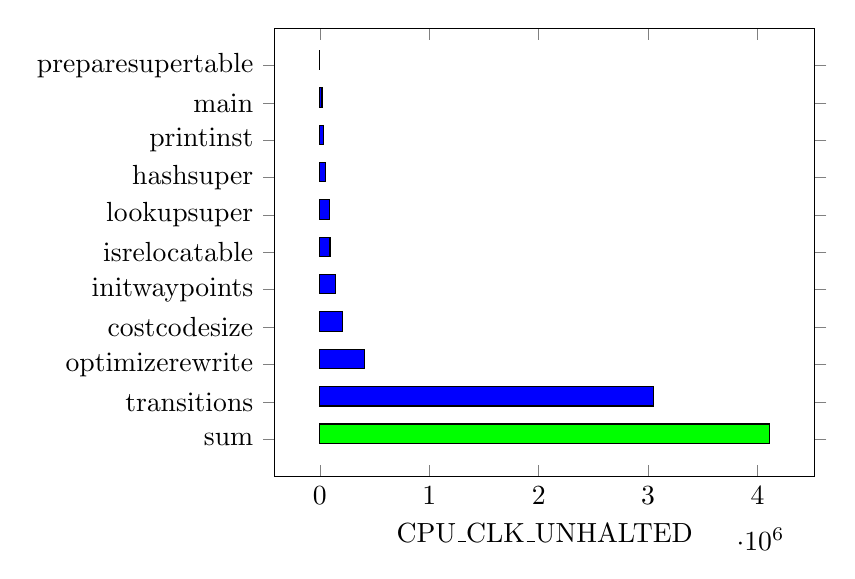
\begin{tikzpicture}
        \begin{axis}[   xbar,
                        symbolic y coords={sum,transitions,optimizerewrite,costcodesize,initwaypoints,isrelocatable,lookupsuper,hashsuper,printinst,main,preparesupertable},
                        xlabel=CPU\_CLK\_UNHALTED,
                        bar width=7pt,
                        bar shift=2pt,
                        ytick=data,
                        point meta=x * 10^7
                    ]
            \addplot+[draw=black, fill=blue] 
            coordinates {
                (3050495,transitions)
                (410243,optimizerewrite)
                (205597,costcodesize)
                (145182,initwaypoints)
                (93162,isrelocatable)
                (92836,lookupsuper)
                (55595,hashsuper)
                (34782,printinst)
                (20346,main)
                (676,preparesupertable)
                (4108914,sum)
            };
            \addplot+[draw=black, fill=green] 
            coordinates {
                (4108914,sum)
            };
        \end{axis}
    \end{tikzpicture}
\end{frame}

\begin{frame}
    \frametitle{Ask not what you can do for your compiler}
    \begin{center} ... ask your compiler what he can do for you.
        \includegraphics[scale=0.4]{jfk.jpg}
    \end{center}
\end{frame}

\begin{frame}
    \frametitle{Ask not what you can do for your compiler}
    \begin{itemize}
        \item -O3 statt -O0
        \item $\Rightarrow$ mass inlining
        \item $\Rightarrow$ unrolling
        \item $\Rightarrow$ a lot of other optimizations
    \end{itemize}
\end{frame}

\begin{frame}
    \frametitle{Ask not what you can do for your compiler}
    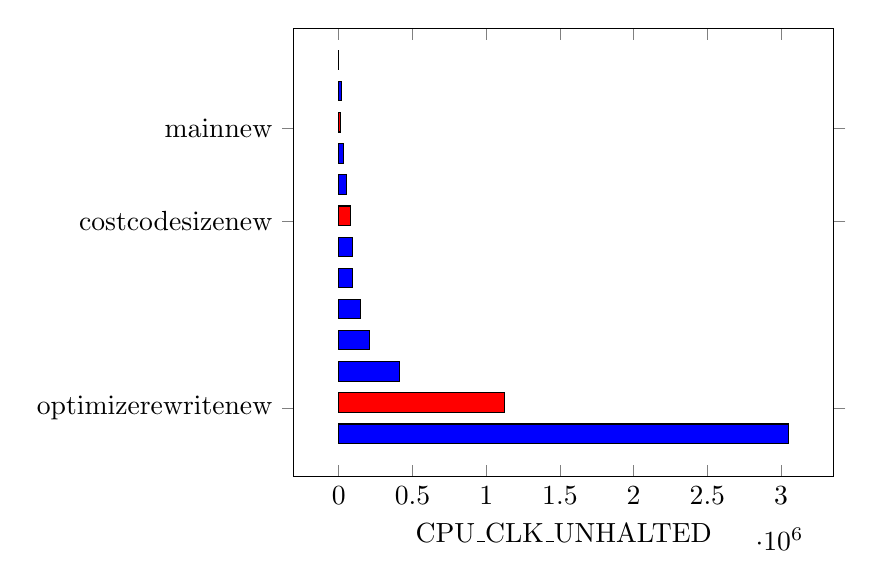
\begin{tikzpicture}
        \begin{axis}[   xbar,
                        symbolic y coords={transitions,optimizerewritenew, optimizerewrite,costcodesize,initwaypoints,isrelocatable,lookupsuper,
                                            costcodesizenew,hashsuper,printinst, mainnew, main, preparesupertable},
                        xlabel=CPU\_CLK\_UNHALTED,
                        bar width=7pt,
                        bar shift=2pt,
                        ytick=data,
                        point meta=x * 10^7
                    ]
            \addplot+[draw=black, fill=red] 
            coordinates {
                (1121706,optimizerewritenew)
                (78016,costcodesizenew)
                (11296,mainnew)
            };

            \addplot+[draw=black, fill=blue] 
            coordinates {
                (3050495,transitions)
                (410243,optimizerewrite)
                (205597,costcodesize)
                (145182,initwaypoints)
                (93162,isrelocatable)
                (92836,lookupsuper)
                (55595,hashsuper)
                (34782,printinst)
                (20346,main)
                (676,preparesupertable)
            };
        \end{axis}
    \end{tikzpicture}
\end{frame}

\begin{frame}
    \frametitle{Ask not what you can do for your compiler}
    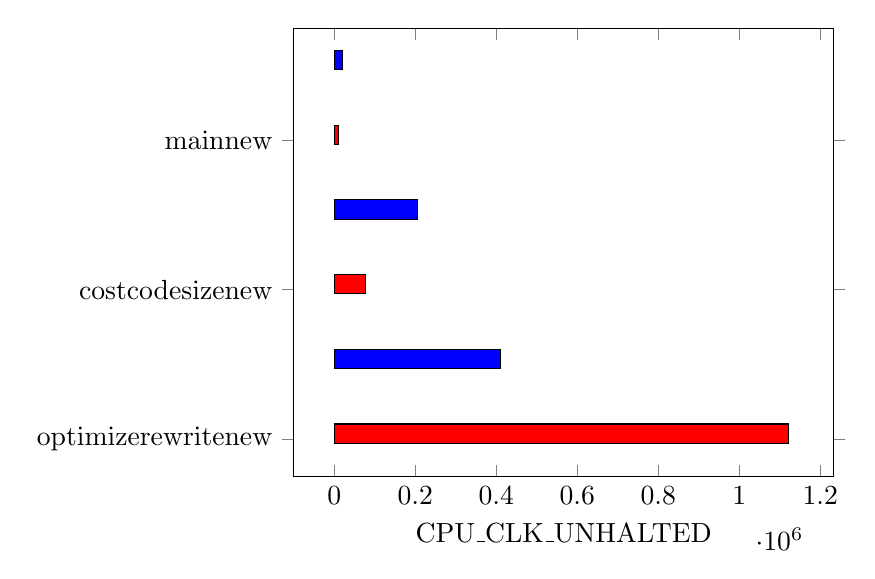
\begin{tikzpicture}
        \begin{axis}[   xbar,
                        symbolic y coords={optimizerewritenew, optimizerewrite, costcodesizenew, costcodesize, mainnew, main},
                        xlabel=CPU\_CLK\_UNHALTED,
                        bar width=7pt,
                        bar shift=2pt,
                        ytick=data
                    ]
            \addplot+[draw=black, fill=red] 
            coordinates {
                (1121706,optimizerewritenew)
                (78016,costcodesizenew)
                (11296,mainnew)
            };

            \addplot+[draw=black, fill=blue] 
            coordinates {
                (410243,optimizerewrite)
                (205597,costcodesize)
                (20346,main)
            };
        \end{axis}
    \end{tikzpicture}
\end{frame}

\begin{frame}
    \frametitle{Ask not what you can do for your compiler}
    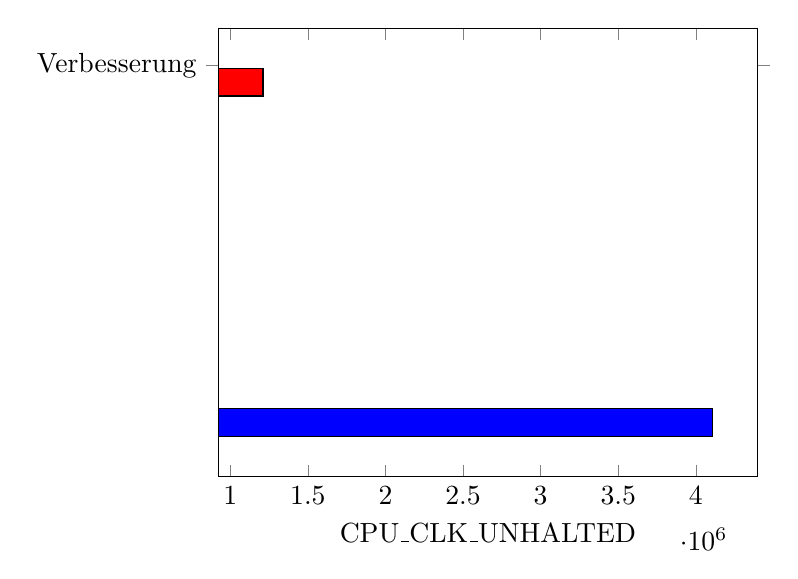
\begin{tikzpicture}
        \begin{axis}[   xbar,
                        symbolic y coords={Ursprung, Verbesserung},
                        xlabel=CPU\_CLK\_UNHALTED,
                        ytick=data
                    ]
            \addplot[draw=black, fill=red] 
            coordinates {
                (1211018,Verbesserung)
            };

            \addplot[draw=black, fill=blue] 
            coordinates {
                (4108914,Ursprung)
            };
        \end{axis}
    \end{tikzpicture}
\end{frame}

\begin{frame}
    \frametitle{Ask not what you can do for your compiler}
    \begin{center} ... but don't ask too much of him.
    \end{center}
\end{frame}

\begin{frame}
    \frametitle{Ask not what you can do for your compiler}
    \begin{itemize}
        \item -funroll-loops
        \item $\Rightarrow$ GCC unrolled Schleifen aggressiv
        \item $\Rightarrow$ Codesize größer
        \item $\Rightarrow$ Performance schlechter
    \end{itemize}
\end{frame}

\begin{frame}
    \frametitle{Ask not what you can do for your compiler}
    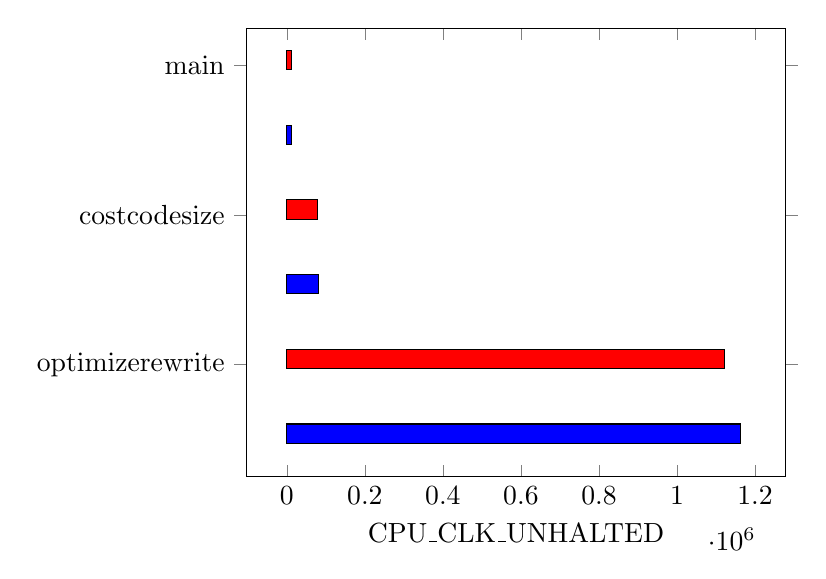
\begin{tikzpicture}
        \begin{axis}[   xbar,
                        symbolic y coords={optimizerewritenew, optimizerewrite, costcodesizenew, costcodesize, mainnew, main},
                        xlabel=CPU\_CLK\_UNHALTED,
                        bar width=7pt,
                        bar shift=2pt,
                        ytick=data
                    ]
            \addplot+[draw=black, fill=red] 
            coordinates {
                (1121706,optimizerewrite)
                (78016,costcodesize)
                (11296,main)
            };

            \addplot+[draw=black, fill=blue] 
            coordinates {
                (1163755,optimizerewritenew)
                (80994,costcodesizenew)
                (11166,mainnew)
            };
        \end{axis}
    \end{tikzpicture}
\end{frame}

\begin{frame}
    \frametitle{Lets actually do something}
    \begin{itemize}
        \item ersetze ss\_cost durch cost\_codesize
        \item cost\_codesize verschwindet komplett
        \item main und optimize\_rewrite marginal besser
    \end{itemize}
\end{frame}

\begin{frame}
    \frametitle{Lets actually do something}
    \begin{center}
    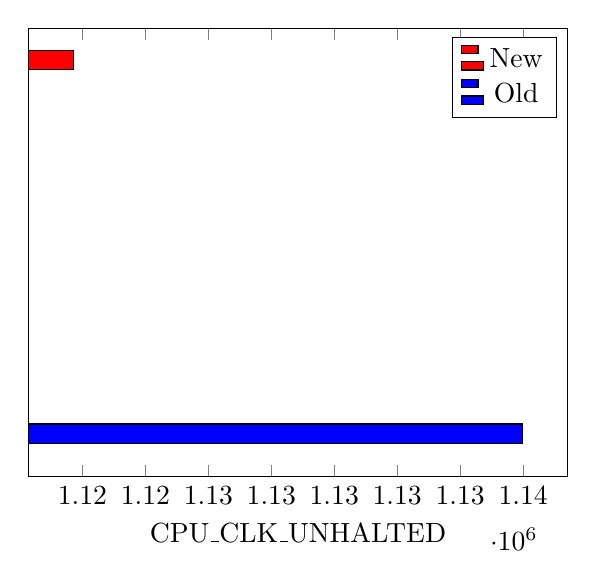
\begin{tikzpicture}
        \begin{axis}[   xbar,
                        xlabel=CPU\_CLK\_UNHALTED,
                        bar width=7pt,
                        bar shift=2pt,
                        ytick=\empty
                    ]
            \addplot+[draw=black, fill=red] 
            coordinates {
                (1121706, 1)
            };
            \addplot+[draw=black, fill=blue] 
            coordinates {
                (1135993, 0)
            };
            \legend{New, Old}
        \end{axis}
    \end{tikzpicture}
    \end{center}
\end{frame}

\begin{frame}
    \frametitle{Lets actually do something}
    \begin{itemize}
        \item Verbesserung main Schleife
    \end{itemize}
\end{frame}

\begin{frame}
    \frametitle{Lets actually do something}
    \begin{center}
    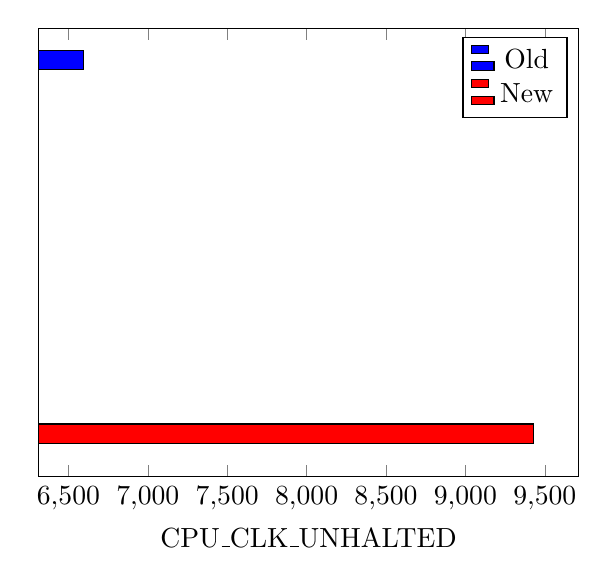
\begin{tikzpicture}
        \begin{axis}[   xbar,
                        xlabel=CPU\_CLK\_UNHALTED,
                        bar width=7pt,
                        bar shift=2pt,
                        ytick=\empty
                    ]

            \addplot+[draw=black, fill=blue] 
            coordinates {
                (6596,1)
            };
            \addplot+[draw=black, fill=red] 
            coordinates {
                (9428,0)
            };

            \legend{Old, New}
        \end{axis}
    \end{tikzpicture}
    \end{center}
\end{frame}

\begin{frame}
    \frametitle{That's it?}
        \begin{itemize}
            \item GCC leistet ganze Arbeit
            \item viele unserer anderen "Optimierungen" schlecht
            \item Codesize kann man noch verbessern
        \end{itemize}
\end{frame}

\begin{frame}
    \frametitle{Codesize}
    \begin{center}
    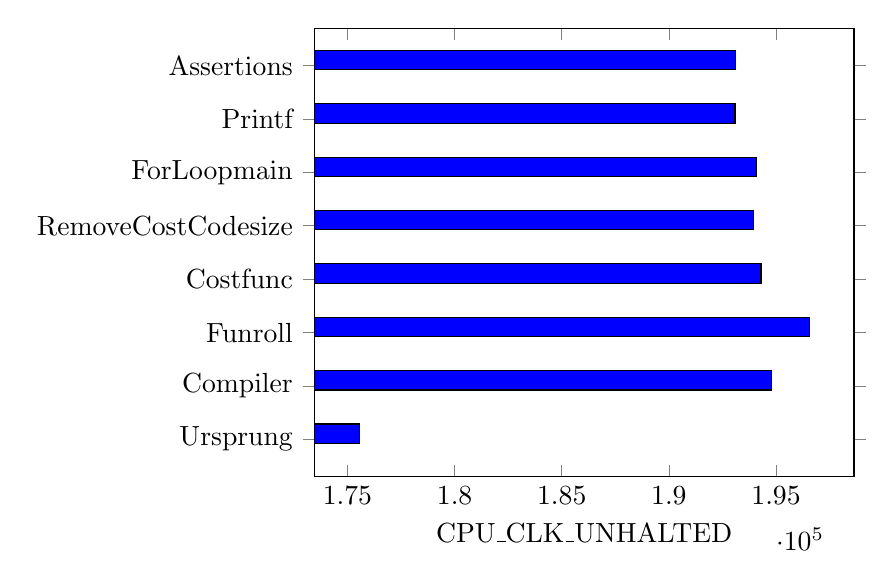
\begin{tikzpicture}
        \begin{axis}[   xbar,
                        symbolic y coords={Ursprung, Compiler, Funroll,
                            Costfunc, RemoveCostCodesize, ForLoopmain, Printf,
                            Assertions},
                        xlabel=CPU\_CLK\_UNHALTED,
                        bar width=7pt,
                        bar shift=2pt,
                        ytick=data
                    ]
            \addplot+[draw=black, fill=blue] 
            coordinates {
                (175555,Ursprung)
                (194789,Compiler)
                (196541,Funroll)
                (194300,Costfunc)
                (193948,RemoveCostCodesize)
                (194084,ForLoopmain)
                (193088,Assertions)
                (193085,Printf)
            };
        \end{axis}
    \end{tikzpicture}
    \end{center}
\end{frame}

\begin{frame}[fragile]
\frametitle{papiex Endergebnisse}

\begin{lstlisting}[caption="Ursprung", captionpos=b]
PAPI_TOT_CYC .......4.27796e+08
PAPI_TOT_INS .......5.30222e+08
PAPI_BR_MSP ........1.28136e+06
PAPI_FP_OPS ........487
\end{lstlisting}

\begin{lstlisting}[caption="Ursprung -O3", captionpos=b]
PAPI_TOT_CYC .......1.44674e+08
PAPI_TOT_INS .......2.2851e+08
PAPI_BR_MSP ........1.04732e+06
PAPI_FP_OPS ........507
\end{lstlisting}

\begin{lstlisting}[caption="Endergebnis", captionpos=b]
PAPI_TOT_CYC .......1.42435e+08
PAPI_TOT_INS .......2.00493e+08
PAPI_BR_MSP ........1.42997e+06
PAPI_FP_OPS ........486
\end{lstlisting}
\end{frame}

\begin{frame}
    \frametitle{Food for Thought}
    \url{http://leto.net/docs/C-optimization.php\#Compute-bound}
    \url{http://people.redhat.com/drepper/cpumemory.pdf}
    \url{http://www.fefe.de/dietlibc/diet.pdf}
    \url{http://www.fefe.de/know-your-compiler.pdf}
\end{frame}

\end{document}
